\documentclass{ctexart}
\usepackage{amsmath}
\usepackage{tikz}
\usepackage{siunitx}
\usetikzlibrary{calc,intersections,arrows.meta}
\definecolor{star}{RGB}{13,171,160}
\begin{document}

\begin{tikzpicture}
    % 五星
    \coordinate (O) at (0,0);
    \coordinate (A) at (0,2);
    \coordinate (B) at ($(O)!1!72:(A)$);
    \coordinate (C) at ($(O)!1!72:(B)$);
    \coordinate (D) at ($(O)!1!72:(C)$);
    \coordinate (E) at ($(O)!1!72:(D)$);
    \path[name path=AC](A) -- (C);
    \path[name path=AD](A) -- (D);
    \path[name path=BD](B) -- (D);
    \path[name path=BE](B) -- (E);
    \path[name path=CE](C) -- (E);

    \path[name intersections={of=AC and BE,by=F}];
    \path[name intersections={of=AC and BD,by=G}];
    \path[name intersections={of=BD and CE,by=H}];
    \path[name intersections={of=AD and CE,by=I}];
    \path[name intersections={of=AD and BE,by=J}];
    \fill[color=star] (A) -- (F) -- (B) -- (G) -- (C) -- (H) -- (D) -- (I) -- (E) -- (J) -- cycle;
\end{tikzpicture}\vspace{2cm}

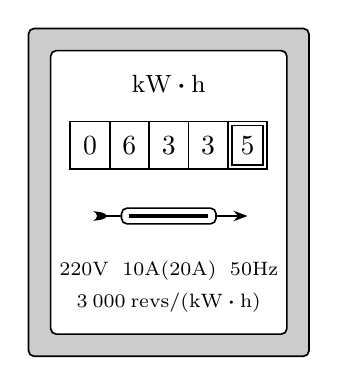
\begin{tikzpicture}[scale=1,transform shape,line width=0.6]
    % 家用机械电能表
    % 外框
    \filldraw[fill=black!20,rounded corners=2pt] (-1.5cm-8pt,-1.8cm-8pt) rectangle (1.5cm+8pt,1.8cm+8pt);
    \filldraw[fill=white,rounded corners=2pt] (-1.5,-1.8) rectangle (1.5,1.8);
    \node at (0,1.38){\small kW\:$\boldsymbol{\cdot}$\:h};
    % 度数
    \foreach \delta in {0,1,2,3,4}{
        \draw (-1.25+0.5*\delta,0.3) rectangle (-0.75+0.5*\delta,0.9);
    }
    \draw (0.8,0.35) rectangle (1.2,.85);
    \node at (-1,0.6){0};
    \node at (-0.5,0.6){6};
    \node at (0,0.6){3};
    \node at (0.5,0.6){3};
    \node at (1,0.6){5};

    % 机械轮
    % 主线条
    \draw[-{Stealth[scale=0.88]},line width=0.6pt] (-1,-0.3) -- (1,-0.3);
    % 尾部
    \filldraw (-1,-0.35) arc [start angle=-90,end angle=90,x radius=0.2,y radius=0.05];
    \filldraw[fill=white,color=white] (-1.06,-0.368) arc [start angle=-90,end angle=90,x radius=0.136,y radius=0.068];
    % 转动轮外框
    \filldraw[fill=white,rounded corners=2pt] (-0.6,-0.4) rectangle (0.6,-0.2);
    % 转动轮
    \draw[line width=1.2pt,rounded corners=.6pt] (-0.5,-0.3) -- (0.5,-0.3);

    % 规格
    \node at (0,-1){\scriptsize 220V\; 10A(20A)\; 50Hz};
    \node at (0,-1.4){\scriptsize 3\:000\:revs/(kW\:$\boldsymbol{\cdot}$\:h)};
\end{tikzpicture}\vspace{2cm}

\begin{tikzpicture}[scale=1,transform shape]
    % 家用电子电能表
    % 外框
    \filldraw[fill=black!20,rounded corners=2pt] (-1.5cm-8pt,-1.8cm-8pt) rectangle (1.5cm+8pt,1.8cm+8pt);
    \filldraw[fill=white,rounded corners=2pt] (-1.5,-1.8) rectangle (1.5,1.8);
    \node at (0,1.38){\small kW\:$\boldsymbol{\cdot}$\:h};
    % 度数
    \foreach \delta in {0,1,2,3,4}{
        \draw (-1.25+0.5*\delta,0.4) rectangle (-0.75+0.5*\delta,1);
    }
    \draw (0.8,0.45) rectangle (1.2,.95);
    \node at (-1,0.7){2};
    \node at (-0.5,0.7){8};
    \node at (0,0.7){1};
    \node at (0.5,0.7){8};
    \node at (1,0.7){6};
    % 灯光
    \filldraw[fill=red!100,draw=white] (-0.3,0.1) circle [radius=2pt];
    \node at (0.2,0.1){\scriptsize 脉冲};
    % 文字
    \node at (0,-0.3){\small 电子式单向电能表};
    % 规格
    \node at (0,-1){\scriptsize 220V\; 10A(20A)\; 50Hz};
    \node at (0,-1.4){\scriptsize 1\:200\:imp/(kW\:$\boldsymbol{\cdot}$\:h)};
\end{tikzpicture}\vspace{2cm}

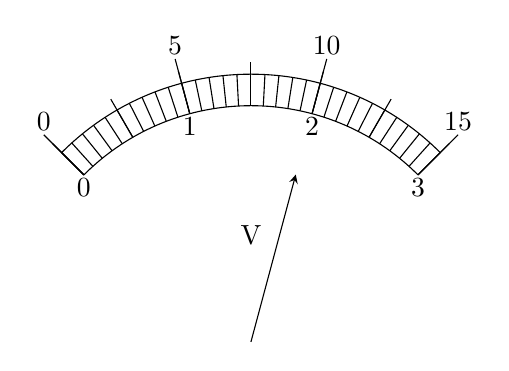
\begin{tikzpicture}
    % 电压表
    \draw (45:3) arc [start angle=45,end angle=135,radius=3];
    \draw (45:3.4) arc [start angle=45,end angle=135,radius=3.4];
    \foreach \smalls in {45,48,...,135}{
        \draw (\smalls:3) -- (\smalls:3.4);
    }
    \foreach \bigs in {45,60,...,135}{
        \draw (\bigs:3) -- (\bigs:3.56);
    }
    \foreach \bbigs/\snum/\bnum in {45/3/15,75/2/10,105/1/5,135/0/0}{
        \draw (\bbigs:3) -- (\bbigs:3.72);
        \node[below=-2pt] at (\bbigs:3){\snum};
        \node[above=-2pt] at (\bbigs:3.72){\bnum};
    }
    \draw[-stealth] (0,0) -- (75:2.2);
    \node at (0,1.36){V};
\end{tikzpicture}\vspace{2cm}

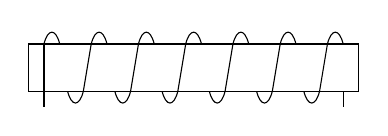
\begin{tikzpicture}
    % 螺线管1(左现右隐)
    \draw (-2,-0.3) rectangle (2.2,0.3);
    % 螺线
    \draw (-1.8,-0.5) -- (-1.8,0.3);
    \foreach \x in {-1.8,-1.2,-0.6,0,0.6,1.2}{
        \draw (\x,0.3) .. controls (\x+0.05,0.5) and (\x+0.15,0.5) .. (\x+0.2,0.3);
        \draw (\x+0.3,-0.3) ..controls (\x+0.35,-0.5) and (\x+0.45,-0.5) .. (\x+0.5,-0.3);
        \draw (\x+0.5,-0.3) -- (\x+0.6,0.3);
    }
    \draw (1.8,0.3) .. controls (1.85,0.5) and (1.95,0.5) .. (2,0.3);
    \draw (2,-0.3) -- (2,-0.5);
\end{tikzpicture}\vspace{2cm}

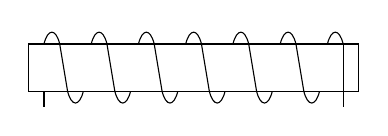
\begin{tikzpicture}
    % 螺线管2(左隐右现)
    \draw (-2,-0.3) rectangle (2.2,0.3);
    % 螺线
    \draw (-1.8,-0.5) -- (-1.8,-0.3);
    \foreach \x in {-1.8,-1.2,-0.6,0,0.6,1.2}{
        \draw (\x,0.3) .. controls (\x+0.05,0.5) and (\x+0.15,0.5) .. (\x+0.2,0.3);
        \draw (\x+0.2,0.3) -- (\x+0.3,-0.3);
        \draw (\x+0.3,-0.3) ..controls (\x+0.35,-0.5) and (\x+0.45,-0.5) .. (\x+0.5,-0.3);
    }
    \draw (1.8,0.3) .. controls (1.85,0.5) and (1.95,0.5) .. (2,0.3);
    \draw (2,0.3) -- (2,-0.5);
\end{tikzpicture}\vspace{2cm}

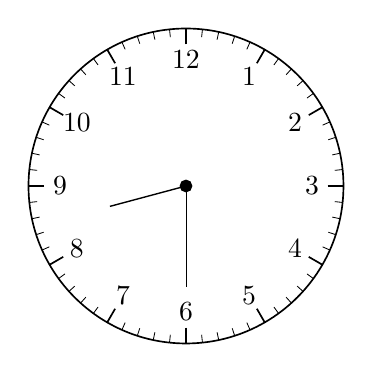
\begin{tikzpicture}[line width=0.6pt]
    % 圆时钟
    \draw (0,0) circle [radius=2cm];
    \foreach \r in {0,6,...,354}{
        \draw[line width=0.3pt] (\r:1.9) -- (\r:2);
    }
    \foreach \r/\n in {0/3,30/2,60/1,90/12,120/11,150/10,180/9,210/8,240/7,270/6,300/5,330/4}{
        \draw (\r:1.8) -- (\r:2);
        \node at (\r:1.6){\n};
    }
    \filldraw (0,0) circle [radius=2pt];
    \draw[line width=0.25pt] (0,0) -- (270:1.28);
    \draw[line width=0.5pt] (0,0) -- (195:1);
\end{tikzpicture}\vspace{2cm}

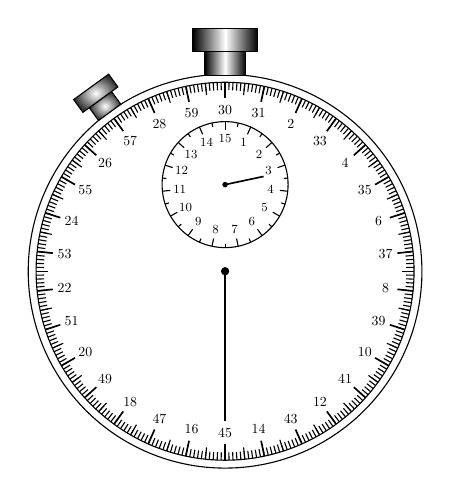
\begin{tikzpicture}[scale=0.5,transform shape]
    % 机械秒表
    % 大表盘
    % 大表盘圆心
    \fill (0,0) circle [radius=3pt];
    % 大表盘框
    \draw (0,0) circle [radius=4.8];
    \draw (0,0) circle [radius=5];
    % 小刻度线
    \foreach \x in {90,88.8,...,-268.8}
        \draw (\x:4.6) -- (\x:4.8);
    % 中刻度线
    \foreach \x in {84,72,...,-264}
        \draw (\x:4.5) -- (\x:4.8);
    % 大刻度线
    \foreach \x in {90,78,...,-258}
        \draw[line width=0.6pt] (\x:4.4) -- (\x:4.8);
    % 刻度标签
    \foreach \x/\y in {78/31,54/33,30/35,6/37,-18/39,-42/41,-66/43,-90/45,-114/47,-138/49,-162/51,-186/53,-210/55,-234/57,-258/59}
        \node at (\x:4.1){\y};
    \foreach \x/\y in {66/2,42/4,18/6,-6/8,-30/10,-54/12,-78/14,-102/16,-126/18,-150/20,-174/22,-198/24,-222/26,-246/28,-270/30}
        \node at (\x:4.1){\y};

    % 小表盘
    % 小表盘圆心
    \fill (90:2.2) circle [radius=2pt];
    % 小表盘框
    \draw (90:2.2) circle [radius=1.6];
    % 大刻度线与刻度标签
    \foreach \x/\y in {66/1,42/2,18/3,-6/4,-30/5,-54/6,-78/7,-102/8,-126/9,-150/10,-174/11,-198/12,-222/13,-246/14,-270/15}{
        \draw[shift={(90:2.2)}] (\x:1.4) -- (\x:1.6);
        \node at ([shift={(90:2.2)}]\x:1.16){\small\y};
    }
    % 小刻度线
    \foreach \x in {78,54,...,-258}
        \draw[shift={(90:2.2)}] (\x:1.5) -- (\x:1.6);

    % 启动/停止按钮
    \draw[left color=black,right color=black,middle color=white] (96:5) rectangle ([yshift=0.6cm]84:5);
    \draw[left color=black,right color=black,middle color=white] ([shift={(-0.3,0.6)}]96:5) rectangle ([shift={(0.3,1.2)}]84:5);
    % 复位按钮
    \draw[shading=radial,inner color=white,outer color=black!80,rotate=36] (94:5) rectangle ([yshift=0.4cm]86:5);
    \draw[shading=radial,inner color=white,outer color=black!80,rotate=36] ([shift={(-0.2,0.4)}]94:5) rectangle ([shift={(0.2,0.8)}]86:5);

    % 大表盘指针
    \draw[line width=0.8pt] (0,0) -- (-90:3.8);
    % 小表盘指针
    \draw[line width=0.6pt,shift={(90:2.2)}] (0,0) -- (12:1);
\end{tikzpicture}\vspace{2cm}

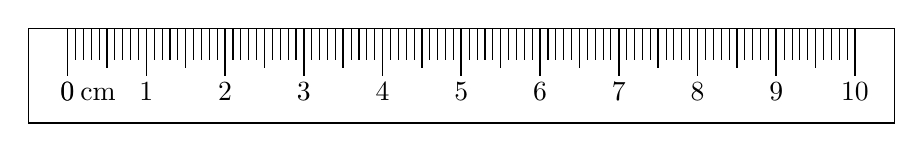
\begin{tikzpicture}
    % 直尺(10 cm)
    \draw (-0.5,-1.2) rectangle (10.5,0);
    \foreach \x in {0,0.1,...,10}
        \draw (\x,-0.4) -- (\x,0);
    \foreach \x in {0,0.5,...,10}
        \draw[line width=0.5pt] (\x,-0.5) -- (\x,0);
    \foreach \x in {0,1,...,10}{
        \draw[line width=0.6pt] (\x,-0.6) -- (\x,0);
        \node at (\x,-0.8){\x};
    }
    \node at (0.26,-0.8){0\:cm};
\end{tikzpicture}\vspace{2cm}

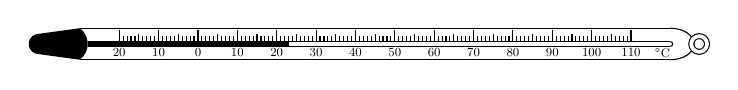
\begin{tikzpicture}[scale=0.5,font=\small,transform shape]
    % 温度计1
    % 外壁
    \draw (-3,0.4) -- (12,0.4);
    \draw (-3,-0.4) -- (12,-0.4);
    \fill (-4.1,0.25) arc [start angle=102.5,end angle=257.5,radius=0.256] -- (-3,-0.4) -- (-3,-0.4) arc [start angle=-53.2,end angle=53.2,radius=0.5] -- cycle;
    \draw (12,-0.4) arc [start angle=-90,end angle=90,x radius=0.6,y radius=0.4];
    \draw[double,double distance=1.36pt] (12.73,0) circle [radius=0.2];
    % 刻度线
    \draw (-2.8,0.06) -- (12,0.06);
    \draw (-2.8,-0.06) -- (12,-0.06);
    \draw (12,-0.06) arc [start angle=-90,end angle=90,radius=0.06];
    \foreach \x in {-2,-1.9,...,11}
        \draw (\x,0.06) -- (\x,0.21);
    \foreach \x in {-2,-1.5,...,11}
        \draw (\x,0.06) -- (\x,0.26);
    \foreach \x/\y in {-2/20,-1/10,0,1/10,2/20,3/30,4/40,5/50,6/60,7/70,8/80,9/90,10/100,11/110}{
        \draw (\x,0.06) -- (\x,0.36);
        \node[below=-2pt] at (\x,-0.06){\y};
    }
    \node[below=-2pt] at (11.8,-0.06){\qty{}{\degreeCelsius}};
    % 水银
    \fill (-2.8,-0.06) rectangle (2.3,0.06);
\end{tikzpicture}\vspace{2cm}

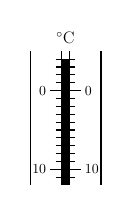
\begin{tikzpicture}[scale=0.5,transform shape]
    % 温度计2
    % 外壁
    \draw (-0.9,1) -- (-0.9,-2.4);
    \draw (0.9,1) -- (0.9,-2.4);
    % 刻度线
    \draw (-0.1,1) -- (-0.1,-2.4);
    \draw (0.1,1) -- (0.1,-2.4);
    \foreach \x in {-2.2,-2,...,0.8}{
        \draw (-0.25,\x) -- (-0.1,\x);
        \draw (0.1,\x) -- (0.25,\x);
    }
    \foreach \x/\y in {0,-2/10}{
        \draw[line width=0.6pt] (-0.4,\x) -- (-0.1,\x) node[pos=0,left=-1pt]{$\y$};
        \draw[line width=0.6pt] (0.1,\x) -- (0.4,\x) node[pos=1,right=-1pt]{\y};
    }
    % 摄氏度符号
    \node[above=2pt] at (0,1){\large\qty{}{\degreeCelsius}};
    % 水银
    \fill (-0.1,-2.4) rectangle (0.1,0.8);
\end{tikzpicture}\vspace{2cm}

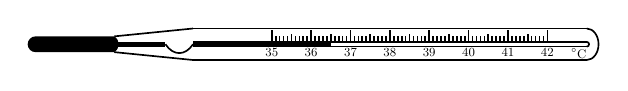
\begin{tikzpicture}[line width=0.6pt,scale=0.5,font=\small,transform shape]
    % 体温计
    % 外壁
    \draw (-2,0.4) -- (8,0.4);
    \draw (-2,-0.4) -- (8,-0.4);
    \fill (-6,0.2) arc [start angle=90,end angle=270,radius=0.2] -- (-6,-0.2) -- (-4,-0.2) .. controls (-3.85,-0.1) and (-3.85,0.1) .. (-4,0.2) -- cycle;
    \draw (-4,0.2) -- (-2,0.4);
    \draw (-4,-0.2) -- (-2,-0.4);
    \draw (8,-0.4) arc [start angle=-90,end angle=90,x radius=0.3,y radius=0.4];
    % 刻度线
    \fill (-4,-0.06) rectangle (-2.7,0.06);
    \draw (-2.7,0) .. controls (-2.5,-0.3) and (-2.2,-0.3) .. (-2,0);
    \draw (-2,0.06) -- (8,0.06);
    \draw (-2,-0.06) -- (8,-0.06);
    \draw (8,-0.06) arc [start angle=-90,end angle=90,radius=0.06];
    \foreach \x in {0,0.1,...,7}
        \draw (\x,0.06) -- (\x,0.21);
    \foreach \x in {0,0.5,...,7}
        \draw (\x,0.06) -- (\x,0.26);
    \foreach \x/\y in {0/35,1/36,2/37,3/38,4/39,5/40,6/41,7/42}{
        \draw (\x,0.06) -- (\x,0.36);
        \node[below=-2pt] at (\x,-0.06){\y};
    }
    \node[below=-2pt] at (7.8,-0.06){\qty{}{\degreeCelsius}};
    % 水银
    \fill (-2,-0.06) rectangle (1.5,0.06);
\end{tikzpicture}\vspace{2cm}

\begin{tikzpicture}[font=\small]
    % 凸透镜
    % 镜面
    \path[name path=c1] ([xshift=-2.6cm]-22:2.8) arc [start angle=-22,end angle=22,radius=2.8];
    \path[name path=c2] ([xshift=2.6cm]158:2.8) arc [start angle=158,end angle=202,radius=2.8];
    \path[name intersections={of=c1 and c2,by={A,B}}];
    \path
      let
        \p1=(A),\p2=(B),
        \n1={2.6cm}
      in
        [draw=dark,fill=light] (\p2) arc [start angle={atan2(\y2,\n1)},end angle={atan2(\y1,\n1)},radius=2.8] -- (\p1) arc [start angle={180-atan2(\y1,\n1)},end angle={180-atan2(\y2,\n1)},radius=2.8];
    % 主光轴
    \draw[dash pattern=on 2pt off 2pt] (-2.6,0) -- (2.6,0) node[above=-1pt,pos=0.2]{主光轴};
    % 光心
    \draw[line width=0.2pt] (0,0) -- (0.5,-0.3) node[pos=1,below=-2pt]{光心};
    \fill[red] (0,0) circle [radius=2pt];
    \node at (12pt,6pt){$O$};
    % 球心
    \fill (-2.6,0) circle [radius=2pt];
    \node[below] at (-2.6,0){$C$};
    \fill (2.6,0) circle [radius=2pt];
    \node[below] at (2.6,0){$C'$};
\end{tikzpicture}\vspace{2cm}

\begin{tikzpicture}[scale=0.8,transform shape]
    % 凹透镜
    % 镜面
    \path[name path=c1] ([xshift=-2.9cm]-22:2.8) arc [start angle=-22,end angle=22,radius=2.8];
    \path[name path=c2] ([xshift=2.9cm]158:2.8) arc [start angle=158,end angle=202,radius=2.8];
    \path[name path=l1] (-0.5,-1.04) -- (0.5,-1.04);
    \path[name path=l2] (-0.5,1.04) -- (0.5,1.04);
    \path[name intersections={of=c1 and l1,by=A}];
    \path[name intersections={of=c1 and l2,by=B}];
    \path[name intersections={of=c2 and l1,by=C}];
    \path[name intersections={of=c2 and l2,by=D}];
    \path
      let
        \p1=(A),\p2=(B),\p3=(C),\p4=(D),
        \n1={2.6cm}
      in
        [draw=dark,fill=light] (\p1) arc [start angle={atan2(\y1,\n1)},end angle={atan2(\y2,\n1)},radius=2.8] -- (\p4) arc [start angle={180-atan2(\y2,\n1)},end angle={180-atan2(\y1,\n1)},radius=2.8] -- cycle;
    % 主光轴
    \draw[dash pattern=on 2pt off 2pt] (-2.9,0) -- (2.9,0) node[above=-1pt,pos=0.2]{主光轴};
    % 光心
    \draw[line width=0.1pt] (0,0) -- (0.5,-0.3) node[pos=1,below=-2pt]{光心};
    \fill[red] (0,0) circle [radius=2pt];
    \node at (12pt,6pt){$O$};
    % 球心
    \fill (-2.9,0) circle [radius=2pt];
    \node[below] at (-2.9,0){$C$};
    \fill (2.9,0) circle [radius=2pt];
    \node[below] at (2.9,0){$C'$};
\end{tikzpicture}
\end{document}

